\section{Technique Knowledge Graph}
\label{sec:tkg}

\subsection{TKG design}

The TKG should take a hierarchical (two-layer) design, namely, system entity (and action) level and TTP level. On system entity level, the TKG looks just like many sub-graphs(TPG) of Provenance Graph.  Every sub-graph represents a TTP and make up the TTP-level TKG. Every TTP node should have one or more inputs and outputs. And we can use these inputs and outputs connect TTPs.


\subsubsection{Layer 1: kill chain layer}

\subsubsection{Layer 2: TTP representation layer}

\subsection{Building the TKG – The Workflow:
}

\begin{figure}
    \centering
    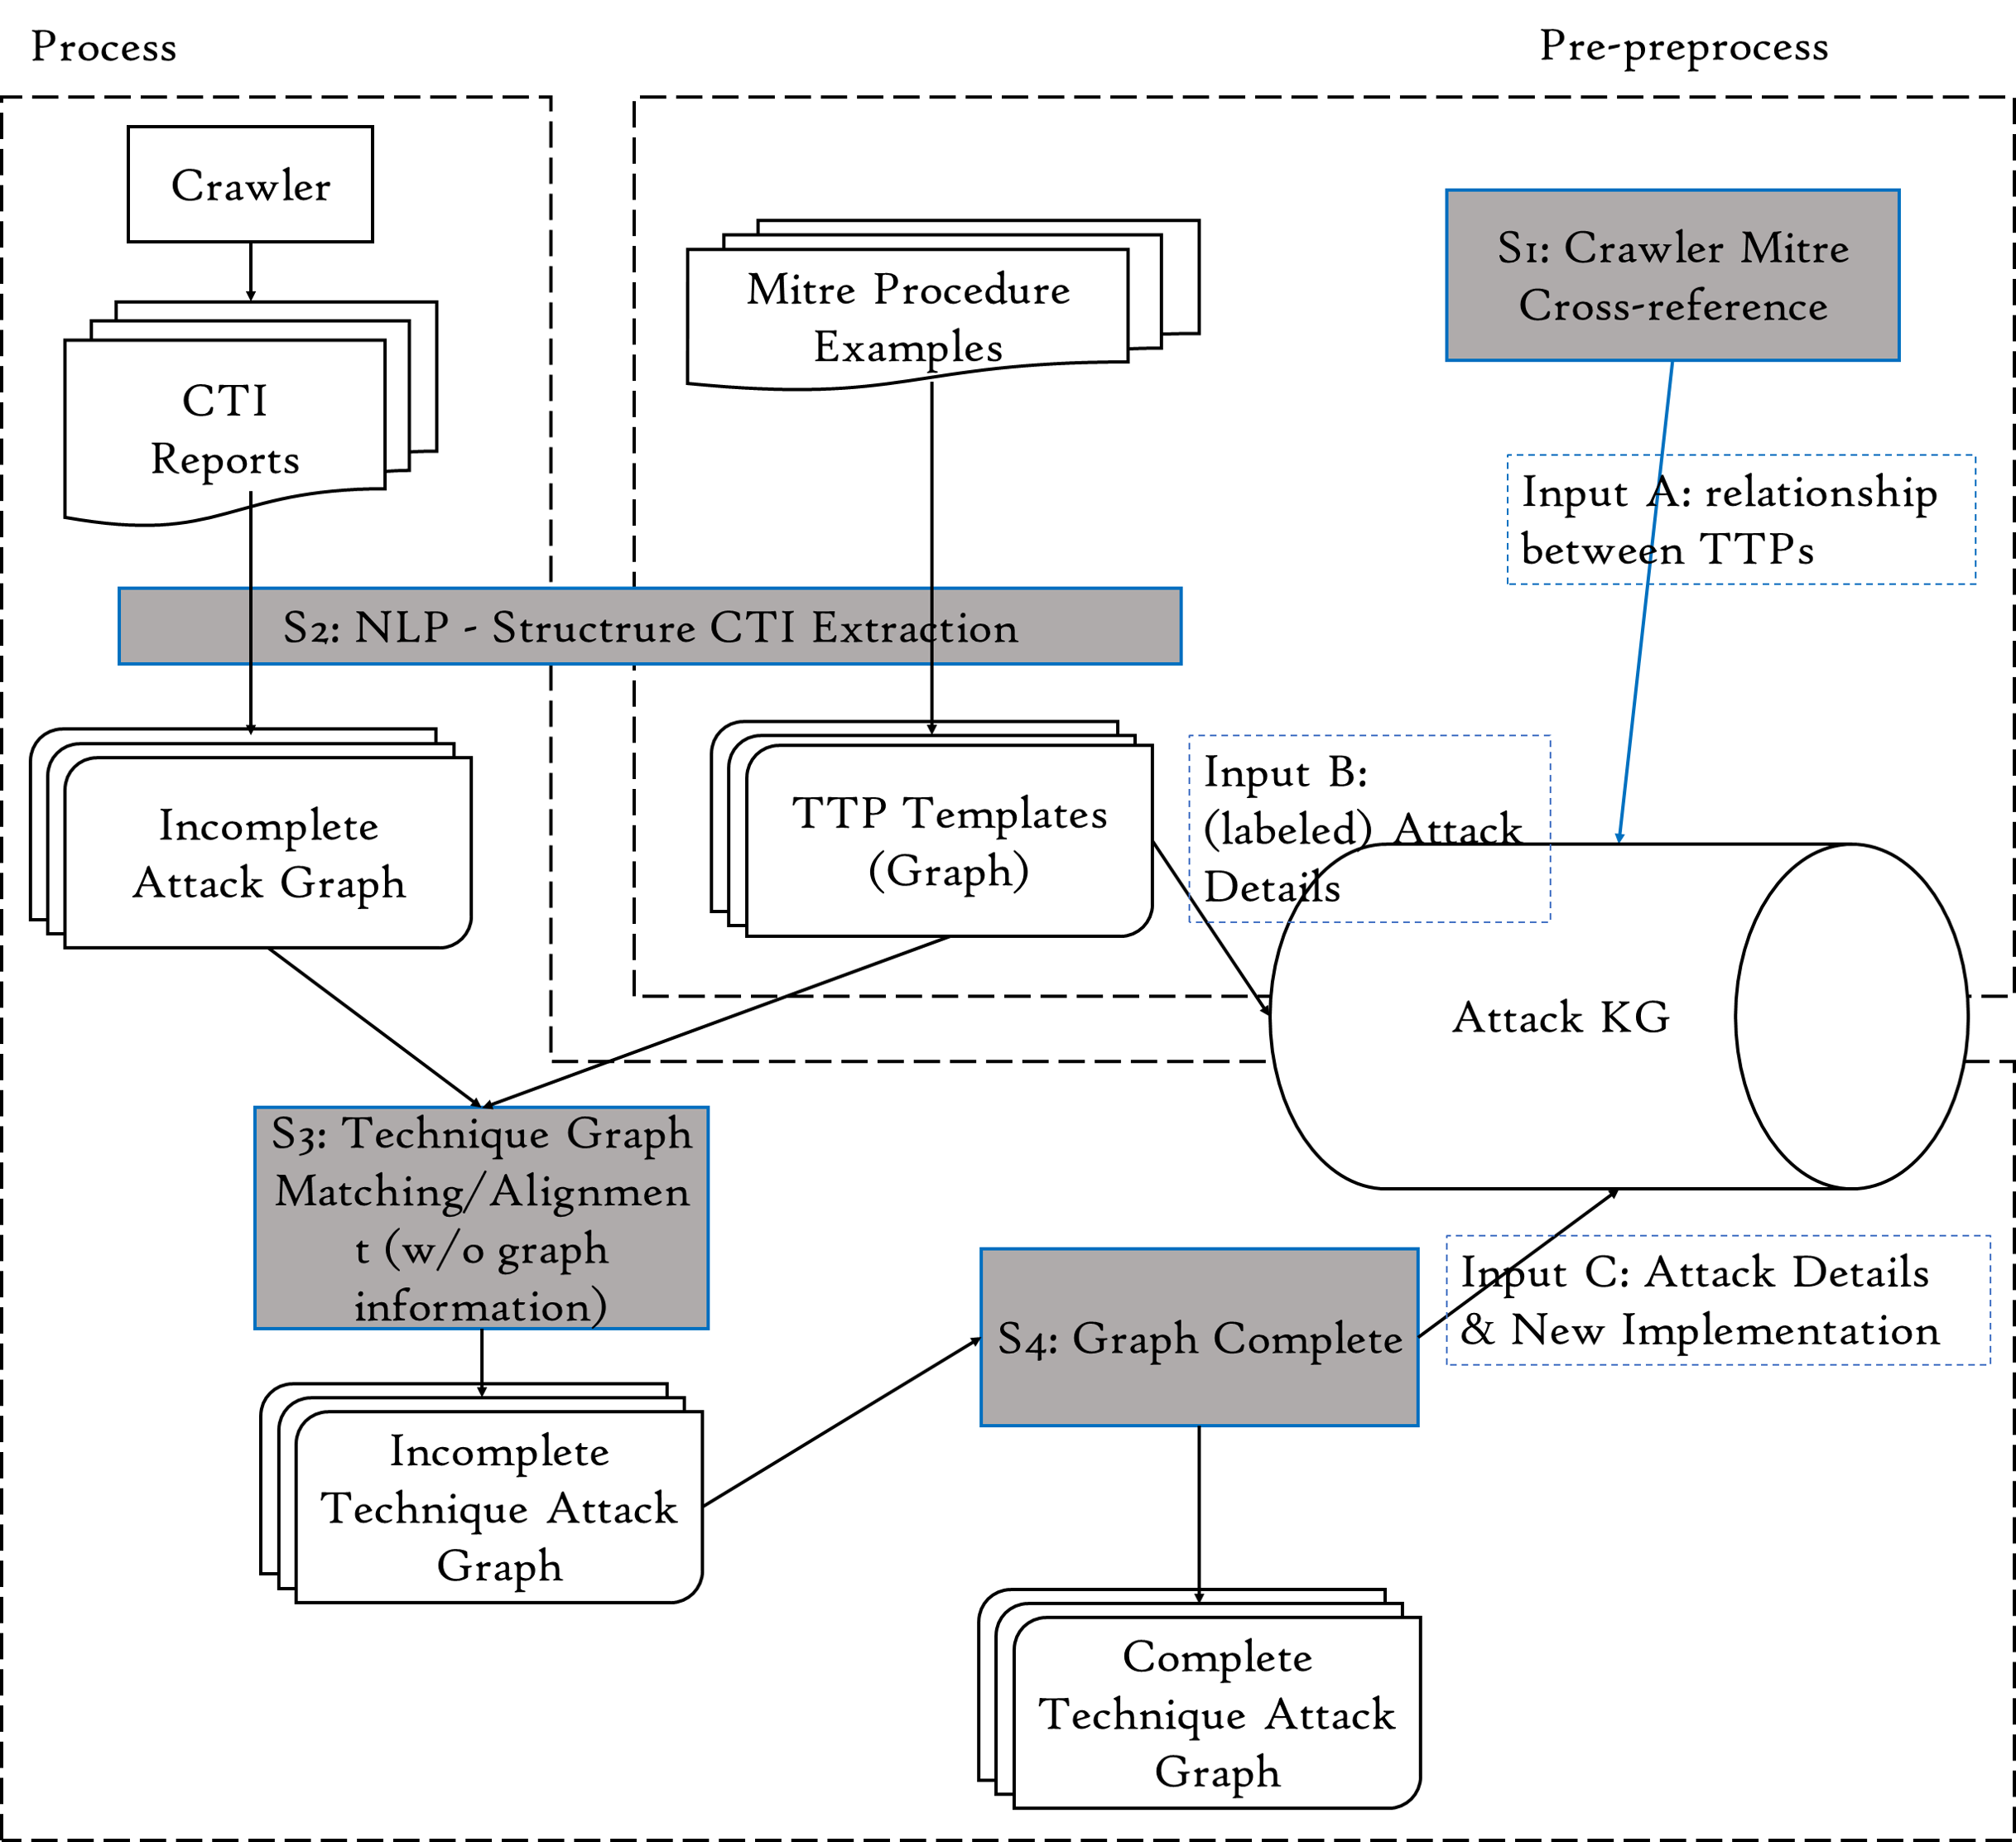
\includegraphics[width=3.5in]{Image/architecture.png}
    \caption{Attack Knowledge Graph Building Process.}
    \label{fig:architecture}
\end{figure}

\subsubsection{NLP-based CTI report parsing: the input is CTI reports and description for all the TTPs (mitre attack)}

\begin{figure}
    \centering
    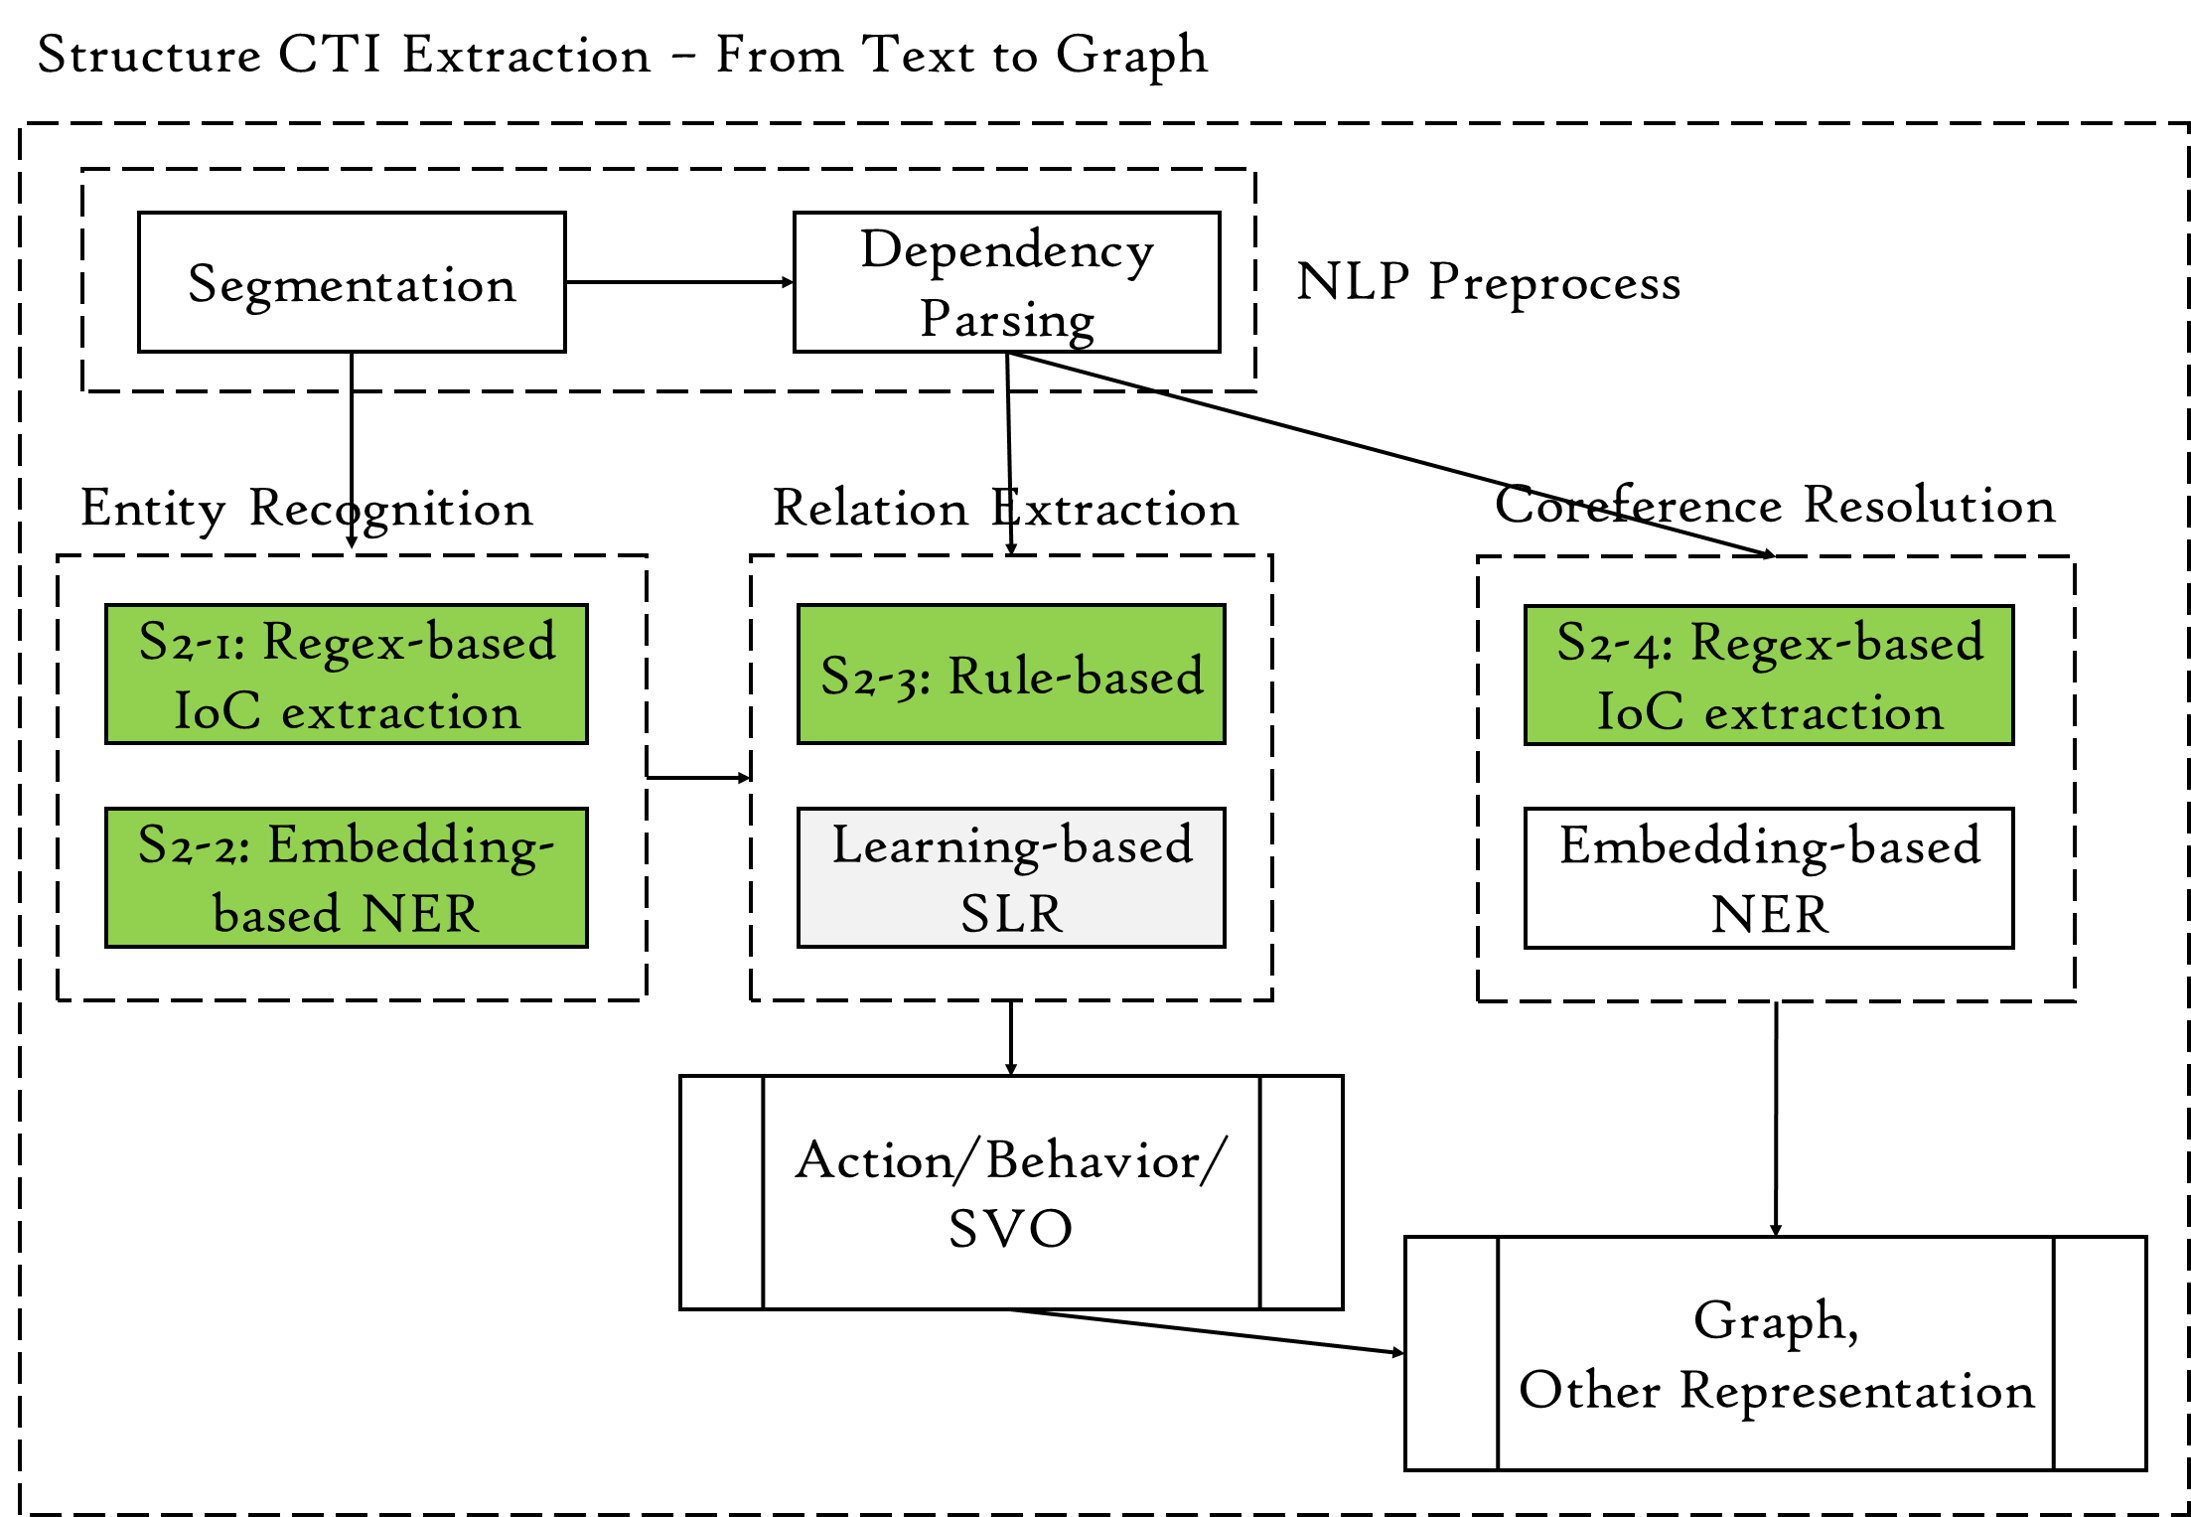
\includegraphics[width=3.5in]{Image/nlp_architecture.png}
    \caption{NLP-based Report Parsiing Process.}
    \label{fig:architecture}
\end{figure}

\textbf{S2-0. Preprocess}.

\textbf{S2-1,2. NLP-based TTP extraction}.

\textbf{S2-3. Relation extraction}.

\textbf{S2-4. Co-reference resolution}.

\textbf{S2-5. Attack graph reconstruction for each TTP segment}.

\subsubsection{TKG initialization-update-loop: the input is subgraphs representing TTPs}

1. Find similar subgraphs in TKG according to TTP, input/output, IoCs, subgraph structure

2. If not match, add subgraphs to the TKG; If match, find the difference and try to abstract a more general model to match both graph.

3. Try to connect the new TTP with other TTPs according to the inputs and outputs.

\subsubsection{Application}
